\begin{figure}[t]
\centering
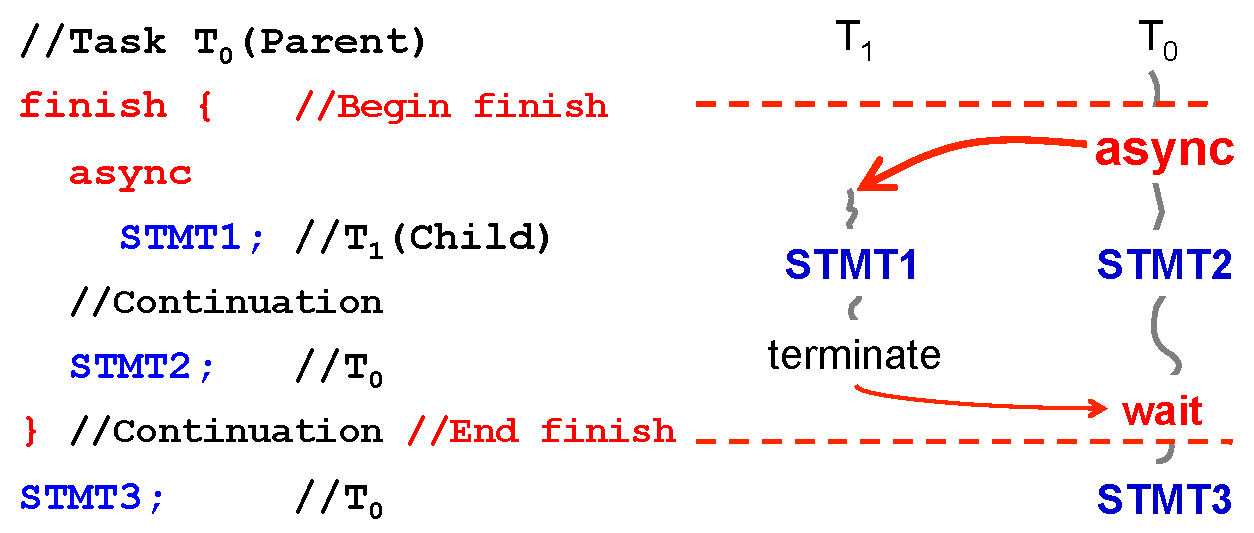
\includegraphics[width=3.25in]{../figs/async-finish}
\caption{An example with {\tt async} and {\tt finish}.}
\label{fig:async-finish}
\end{figure}


\section{Habanero Programming Model}

The Habanero programming model is built around a task-parallel view of
concurrency \cite{Cave:2011:HNA:2093157.2093165}. \figref{fig:async-finish} illustrates Habanero in its
simplest form \cite{Cave:2011:HNA:2093157.2093165}.

The \texttt{async}-construct is a mechanism for
creating a new asynchronous task: {\tt async}
$\langle${\em stmt}$\rangle$ causes the calling task (i.e., the
parent) to create a new child task to execute {\em
  $\langle$stmt$\rangle$} (logically) in parallel with the parent
task. {\em $\langle$stmt$\rangle$} can read or write any data in the
heap and can read (but not write) any local variable belonging to the
parent task's lexical scope. The task created by any
\texttt{async}-construct is scheduled at the point it is declared in
the program.

The \texttt{finish}-construct is a generalized join operation for
collective synchronization: {\tt finish} $\langle${\em
  stmt}$\rangle$ causes the parent task to execute {\em
  $\langle$stmt$\rangle$} and then wait until all tasks created within
{\em $\langle$stmt$\rangle$} have completed, including transitively
created tasks.  Each dynamic instance of a task has a unique {\em
  immediately-enclosing-finish} (IEF) during program execution. That IEF is the
innermost {\tt finish}-construct containing the task.  There is an implicit {\tt
  finish}-construct surrounding the entry point of the program so the program only terminates after
all tasks have completed.

A computation graph illustrating the semantics of the \texttt{async}
and \texttt{finish} constructs is on the right side of
\figref{fig:async-finish}. In the graph, task $T_0$ enters the
\texttt{finish}-construct, creates task $T_1$ at the
\texttt{async}-construct, and then continues on to
\texttt{STMT2}. After \texttt{STMT2}, $T_0$ waits for $T_1$ to
complete before moving on to \texttt{STMT3}. Note that \texttt{STMT1}
and \texttt{STMT2} are not ordered by the semantics and represent
parallel execution.

Habanero supports more advanced forms of tasking beyond creation and
collective synchronization. The \texttt{isolated}-construct, {\tt isolated}~$\langle${\it
  stmt1}$\rangle$, ensures that $\langle${\it stmt1}$\rangle$ is
evaluated in mutual exclusion with all other {\tt
  isolated}-constructs.  There are two subtle nuances in the Habanero
model for the \texttt{isolated}-construct:
\begin{compactenum}
\item The construct ensures mutual exclusion between \texttt{isolated}-constructs and not mutual exclusion on a particular memory location. Mutual exclusion on a particular memory location is implemented by wrapping operations on that memory location in \texttt{isolated}-constructs. 
\item Any Habanero implementation may relax mutual-exclusion between
  \texttt{isolated}-constructs as long as the constructs do not
  interfere with one another. Interference in this context means that
  multiple \texttt{isolated}-constructs access a common memory
  location and at least one of those accesses is a write.
\end{compactenum}

The \texttt{future}-construct lets tasks
return values to other tasks: \textbf{future} {\em f} $=$ \textbf{async}
  $\langle${\em expr}$\rangle$ creates a new child task to evaluate $\langle${\em expr}$\rangle$.  The local
variable {\em f} contains a \emph{future handle} to the newly created
task that can be used to obtain the value produced by $\langle${\em expr}$\rangle$. The blocking operation {\em f.get()} returns that value when the
child task completes.

The most complex construct in the Habanero model is the
\textit{phaser} \cite{Shirako:2008:PUD:1375527.1375568}. A phaser is a form of a barrier that provides
point-to-point fine-grain synchronization between tasks to coordinate
their movement through \emph{phases} of computation. Like barriers, phasers order execution of
portions of the program into phases and restrict tasks from
entering the next phase until the current phase is complete. Unlike
barriers though, phasers allow tasks to specify point-to-point relationships on
multiple phasers, and tasks can dynamically join or leave the phaser.

Tasks register with an instance of a phaser, and on registration,
declare the mode that control how that task
synchronizes relative to other tasks registered on the same
barrier. Synchronization takes place with the \texttt{next}-construct
which may block depending on the state of the phaser, and on how the task is registered with the phaser.
\begin{compactitem}
\item \texttt{SIG}: signal registration means all tasks that have designated themselves as signalers must signal the phaser
in order for the phase to advance.  The \texttt{next}-construct for a signal-only task signals the phaser and immediately advances to the next phase.  The phaser remembers each phase completed by any task.
\item \texttt{SIG\_WAIT}: \emph{signal-wait} registration means the task signals the phaser and then waits for other tasks to complete the phase. This registration mode functions like a traditional barrier. The \texttt{next}-construct for a signal-wait task reports phase completion and then blocks for the other signalers to complete the phase too.
\item \texttt{WAIT}: \emph{wait} registration means that the task blocks at the \texttt{next}-construct until the phase advances. 
\end{compactitem}
Phasers may also be bounded to specify slack in the number of phases that may separate
waiters and signalers so signalers can work ahead of waiters
up to a bound.\footnote{Omitted in this presentation of phasers is the ability of a single task to execute constructs after the end of one phase and before the start of the next phase.}

Habanero includes several other constructs such as
\texttt{foreach}-constructs, \texttt{forall}-constructs, \emph{data
  driven futures}, \emph{actors}, etc. most of which are syntactic
sugar for the presented constructs.

